\chapter{Method}\label{chapter:method}


As already stated in the previous chapters, the proposed approach is an online, modular, semi-supervised, DL based tracker. Single shot unknown object segmentation networks often follow an encoder/ decoder structure. Semi-supervised DL based trackers on the other hand typically require more sophistication in the model architecture. 
% \comWB{maybe shortly say why (and/or move a paraphrased version of the last sentence of this paragraph here. then you also dont need the "a short description of the role of each module ...")} 
The proposed method comprises four key components: an image feature encoder, a decoder, a past frame encoder and a matching module. 
% \comWB{i see where you want to go with your argumentation, but maybe rephrase it a bit - i first understood it that we 'just' add an encoder to instr to get tracking to work} 
Crucially, a matching mechanism is utilised to estimate similarity between encodings from previous and the current frame and to feed the decoder with more temporally consistent encodings that combine information from the previous and current frame. \par

A short description of the role of each module encountered in the proposed architecture follows:

\begin{itemize}
    \item The \textbf{image feature encoder} extracts feature representations of the current frame. 
    %\comWB{just '... extract feature representations from past frames'?}.
    \item The \textbf{past frame encoder} 
    %\comWB{maybe its time to rename this?} 
    encodes past frame information to ensure temporal consistency. In some model variations past information is obtained by combining high level information from ground truths/predictions and previous feature maps encoded with the image feature encoder.
    \item The \textbf{matching block} matches the past frame features and current feature map in a more informed and temporally consistent feature map. 
    % \comWB{maybe rephrase; this mustn't always be the case}
    \item The \textbf{decoder} decodes the processed feature map into binary segmentation masks (one binary mask for each tracked object and the background). 
    %\comWB{background? or is that also tracked?}).

\end{itemize}


\begin{figure}
  \centering
  \begin{tabular}{@{}c@{}}
    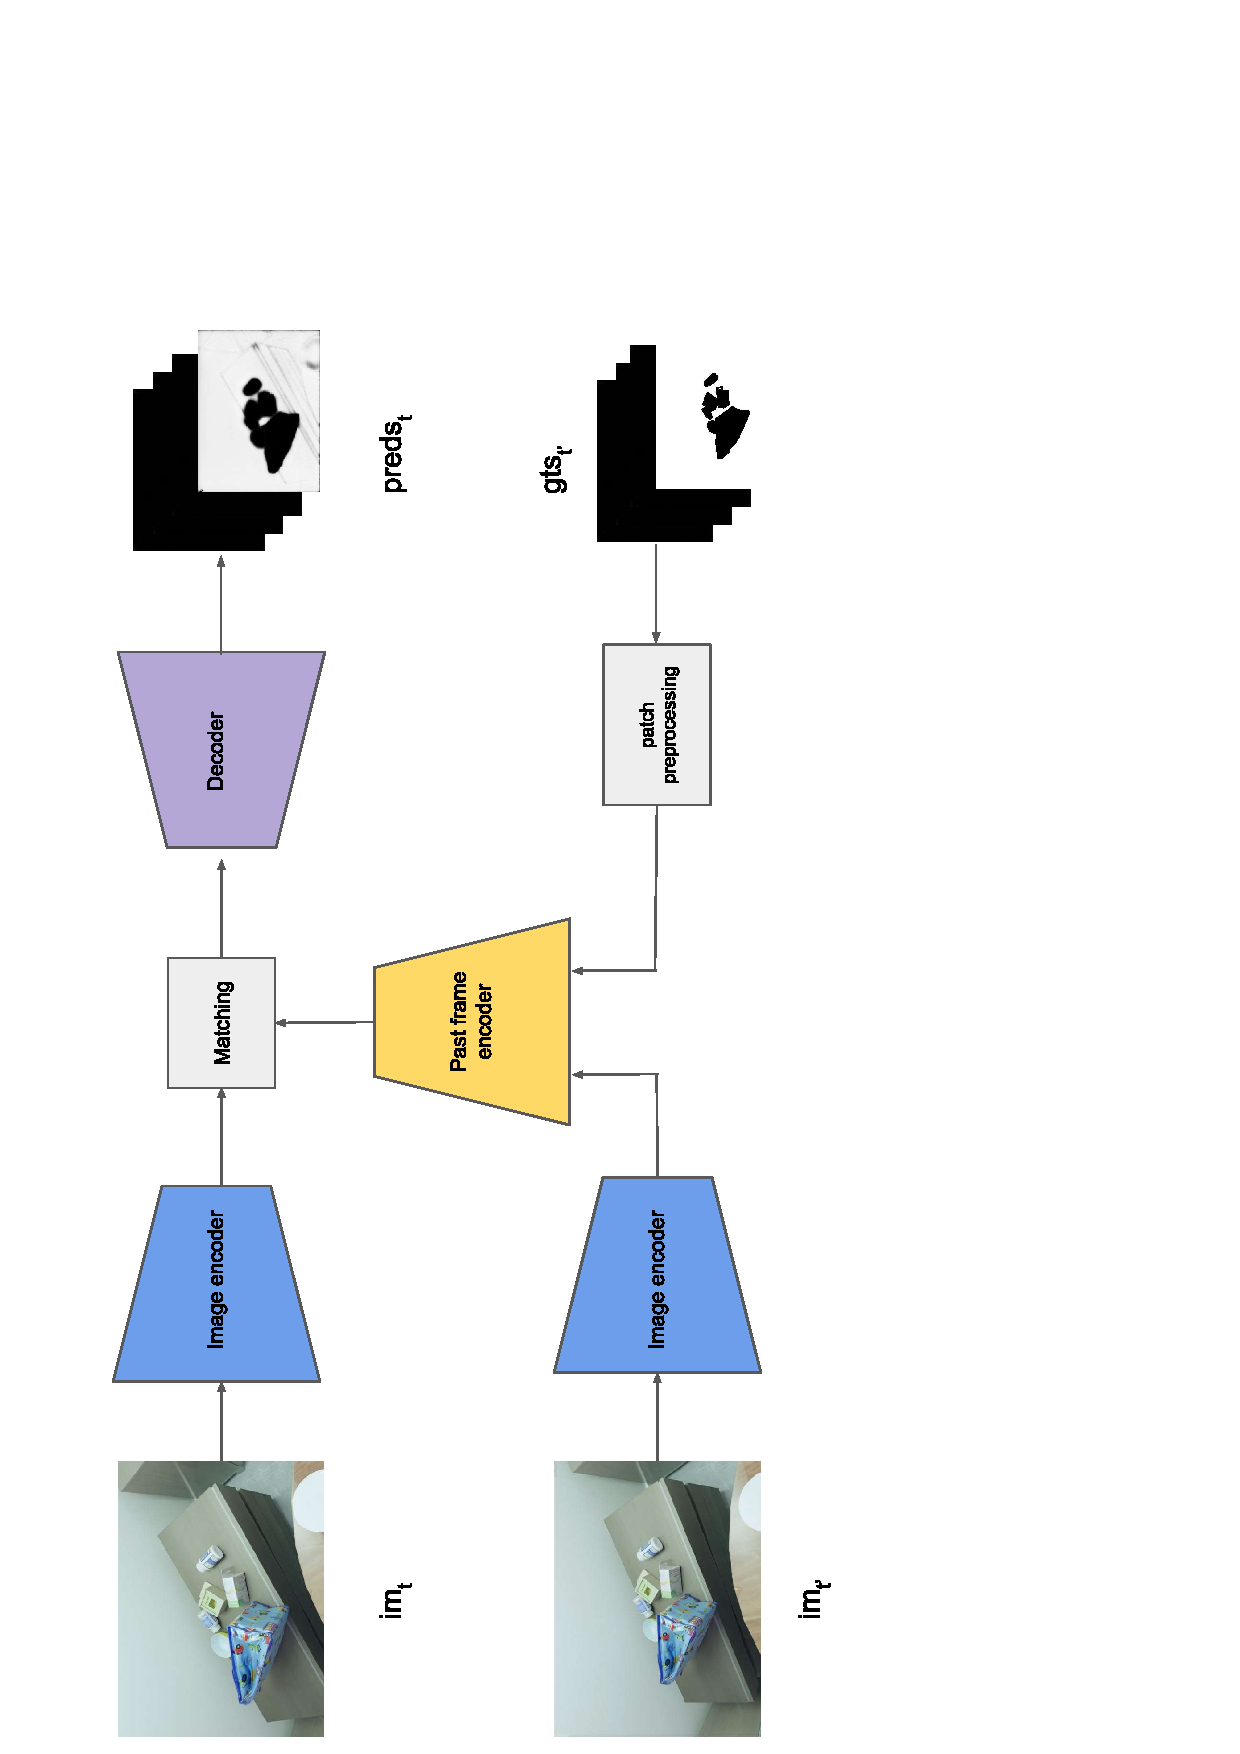
\includegraphics[ angle =-90, 
     trim={ 0 0 6cm 5cm}, width=0.90\linewidth]{figures/03_method/modular_overview_gts.pdf}\\[\abovecaptionskip]
    \small (a) Model overview using past frame ground truths for initialisation
  \end{tabular}

  \vspace{0.5cm}

  \begin{tabular}{@{}c@{}}
    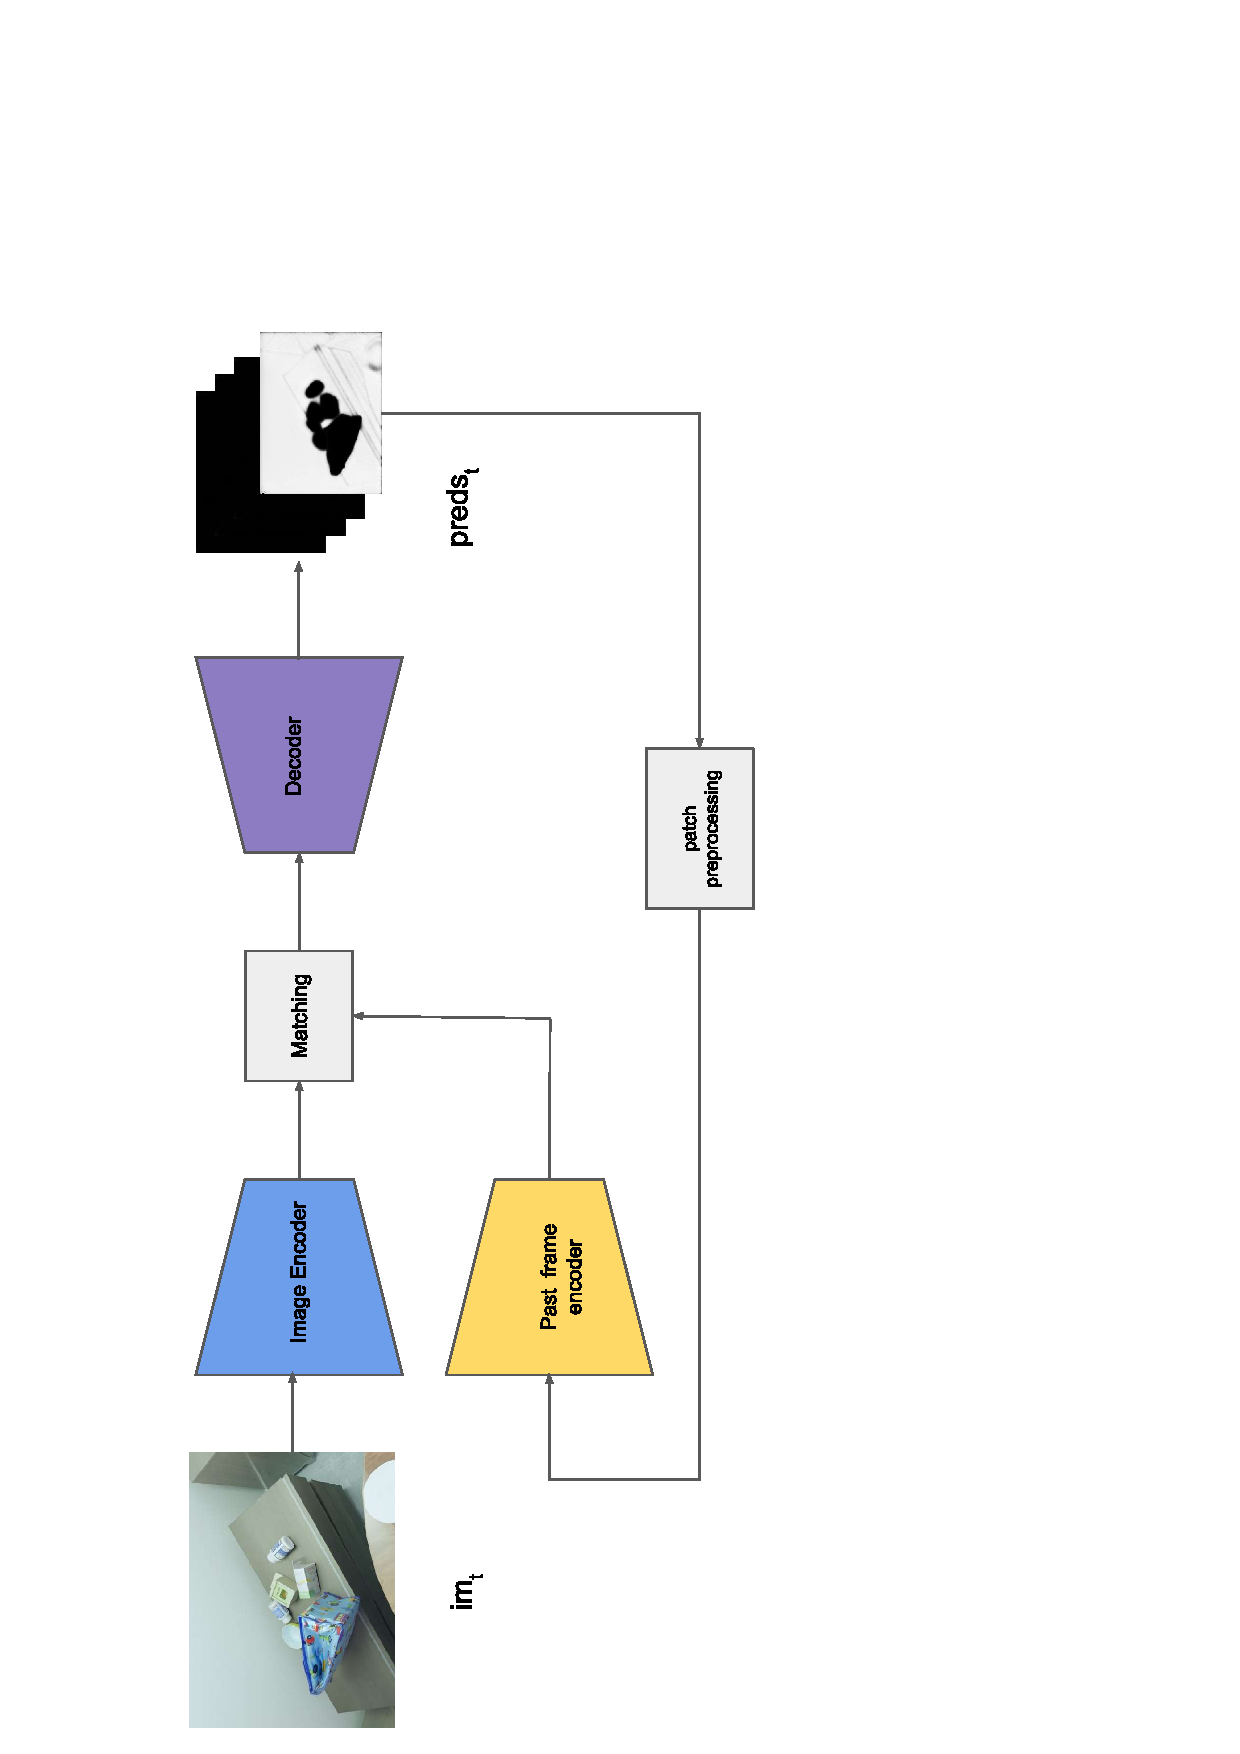
\includegraphics[ angle =-90, 
     trim={ 0 0 7cm 5cm}, width=.90\linewidth]{figures/03_method/modular_overview_preds.pdf}\\[\abovecaptionskip]
    \small (b) Model overview using past frame predictions for initialisation
  \end{tabular}
    
  \caption{Model overview with different initialisation types}
\caption*{Note that $t$ refers to the current frame and $t'$ to the past frame in a sequence of total length T}
  \label{fig:model_overview}
\end{figure}

A modular overview of the proposed method is provided in \figref\ref{fig:model_overview}. During training, tracking is initialised based on the ground truth masks from a past frame. During inference, initialisation can be either performed via a provided past frame ground truth or predictions from another DL network. After initialisation and for the rest of the sequence length, past information is propagated via the predictions from the preceding frame.\par 

In the following sections, more details about the sub-modules encountered in the proposed architecture are provided. For the image feature encoder a transformer based backbone was preferred and not further ablated. For the rest of the modules, different options were investigated and compared with regard to their performance and computational cost in \autoref{chapter:Results}.  \par


\section{Model overview}
\subsection{Image feature encoder}
The image feature encoder block converts an RGB image input to a set of multi-dimensional feature maps. It is used to encode the current input image frame, but also the past image frame for some variants of the past frame encoder. Theoretically, any standard image processing backbone, CNN or transformer based, can potentially be used as image feature encoder. In practice, the SegFormer-B3 \parencite{segformer} backbone was preferred, due to its superior performance with less learnable parameters compared to the popular ResNet-101 \parencite{resnet}. \par

%TODO: give particulars for the segformer version we use (layers, num of learnable parameters, that kind of stuff!)
The SegFormer-B3 belongs to the broader category of transformer based backbones, first introduced by \parencite{dosovitskiy2020vit}. Transformer-based backbones generally lack the inductive biases present in CNNs and require longer pre-training to converge to meaningful representations \parencite{dosovitskiy2020vit}. 
%\comWB{ref missing} 
However, the more elaborate variants of transformer based backbones present superior performance to CNNs for example by following a hierarchical structure in the encoder like in the case of the SegFormer \parencite{segformer} or a hierarchical design with a shifted window strategy like in the case of the Swin family Transformers \parencite{swin}. 
% \comWB{i think if you mention the lack of inductive bias as a downside you should (at least shortly) mention why the newer versions perform better, or how they solve this problem (if it's why the newer variances perform better)}. 
A short description of the SegFormer-B3 backbone encoder follows.\par

% \comWB{for the past frame encoders you have nice subsections separating them, could you do for the segformer here the same? maybe makes it more readable}
The input image of size H × W × 3 is first divided into patches of size 4 × 4 instead of 16 x 16 like in the case of ViT. This designer choice is generally more suitable for the dense prediction task of video object segmentation \parencite{dosovitskiy2020vit}. Then the resulting patches are led to the hierarchical Transformer encoder resulting to multi-level features at different scales of the original image size {1/4, 1/8, 1/16, 1/32}. Depending on the type of matching performed in the matching module, all resulting intermediate feature maps may be involved or just the final output of the encoder at scale 1/32.\par

The transformer block used repeatedly in the encoder consists of three sub modules: an Efficient self-attention block, a Mix-FFN (Feed Forward Network) block
%(\comWB{explain abbrev}) 
and an Overlap Patch Merging block. Efficient self-attention reduces the complexity of the attention mechanism and thus renders attention computation on large image resolutions feasible. The Mix-FFN block is proposed as a data-driven positional encoding mechanism, combining a 3 × 3 convolution and
an \gls{MLP} into each FFN block. Positional encoding mechanisms are typically used along with attention mechanisms to retain positional information of the sequence, which is lost after the attention operation. Finally, Overlapped Patch Merging has a similar effect to a pooling operation and is used to shrink hierarchical feature maps. \par

%\TODO{explain better positional encodings and  Overlapped Patch Merging }

Efficient attention was first introduced in \parencite{pyramid_vision} and involves a spatial reduction operation that reshapes the input sequences to sequences of smaller input size, resulting in less attention operations. The formulas for efficient attention are provided in \eqref{eq:eff1}, \eqref{eq:eff2} and \eqref{eq:eff3} where $K$ the keys, $Q$ the queries, $V$ the values and $d_{head}$ the hidden dimension same as in classic attention mechanism introduced in \parencite{AttentionIsAllYouNeed}. All $K$, $Q$, $V$ are tensors of shape $\mathbb{R}^{NxC}$ where $N = H x W $ is the length of the sequence equal to the flattened patch spatial dimensions. The length of the sequences $N$ is reduced by applying a reduction rate $R^2$ to all three $K$, $Q$, $V$ as indicated for $K$ in \eqref{eq:eff2}. The original tensors can be recovered by applying \eqref{eq:eff3}.

\begin{gather}
    Attention(Q, K, V) = Softmax(\frac{QK^T}{\sqrt{d_{head}}})V \label{eq:eff1}\\
    K' = Reshape(\frac{N}{R^2}, C R^2)(K) \label{eq:eff2}\\
    K = Linear(C R^2, C)(K') \label{eq:eff3}
\end{gather}

For more details on the Mix-FFN and the Overlapped Patch Merging blocks we refer the reader to \parencite{segformer}.
%\comWB{parencite or not}

\vspace{5mm}
\subsection{Past frame encoder}

In the course of this work, three main variants for the past frame encoder are examined. In the first case, the backbone 
% \comWB{either remove the "'", or also use them later e.g. in matching section etc. personally i like writing stuff italic the first time, but its up to you} 
past frame encoder is built on an identical SegFormer-B3 block with the image feature encoder with different weights. The two other options are more lightweight alternatives to the 'backbone' image encoder, the motion-based 'bounding box encoder' and the appearance-based 'mask encoder'. A more detailed description of the three examined encoder options follows.



\subsubsection{Backbone encoder}
%\subsubsection{Patch preprocessing}
In the first past frame encoding case, the encoder design is very similar to the image feature encoder. More specifically, a siamese SegFormer-B3 encoder is used with different weights than the image feature encoder SegFormer-B3. The past frame encoder inputs result from masking a past input image with either the ground truth (during training) or the predicted binary masks from the same previous frame (during inference). The result is an RGB image that involves only the highlighted object of interest, see \figref\ref{fig:standard_patch}. The resulting patches are then downsampled from 480x640 to 120x160 with bicubic interpolation. An overview of this model variant is provided in \figref\ref{fig:detailed_model_backbone}.
%TODO: add patches visualization
%superposition basically by computing img*mask

%can also be combined with multi res matching unlike the other two patch encoder options 
\begin{figure}[!ht]
    \subfloat[Example overlay\label{subfig-1:standard_patch}]{%
      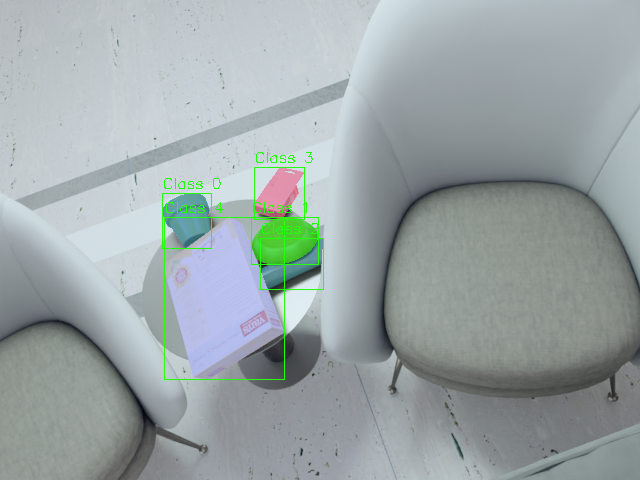
\includegraphics[width=0.30\textwidth]{figures/03_method/example_overlay.png}
    }
    \hfill
    \subfloat[Example binary mask\label{subfig-2:standard_patch}]{%
      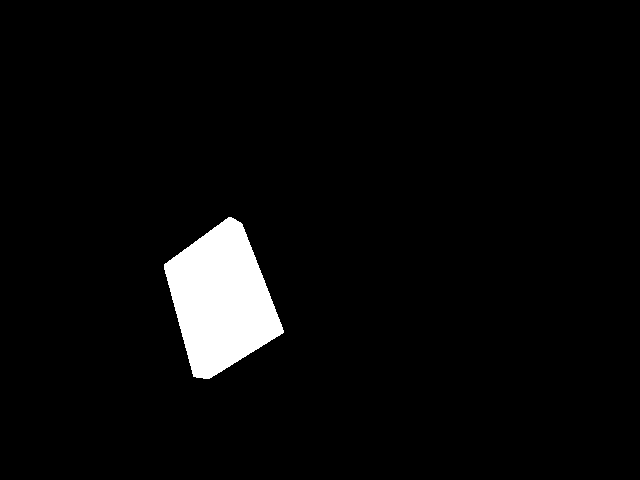
\includegraphics[width=0.30\textwidth]{figures/03_method/example_binary_mask.png}
    }
    \hfill
    \subfloat[Example patch\label{subfig-3:standard_patch}]{%
      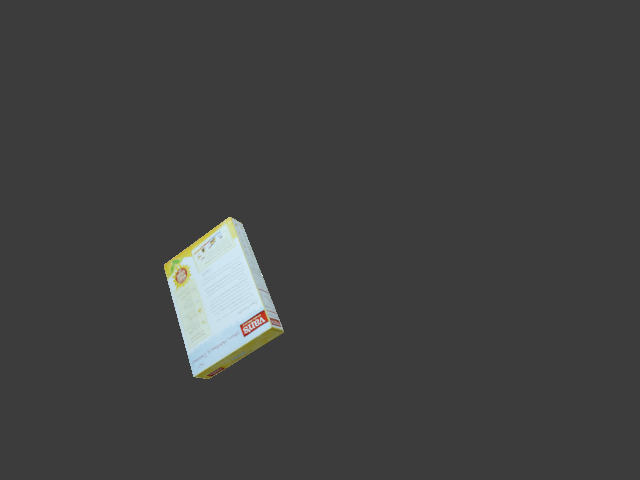
\includegraphics[width=0.30\textwidth]{figures/03_method/example_patch.png}
    }
    \caption{Patch generation for backbone encoder 
    }
    \label{fig:standard_patch}
  \end{figure}
  % \comWB{very picky, but i think you dont have bboxes for the other visualizations, right? if its easy to keep it consistent i would do that}
%\subsubsection{Encode patches}

In general, this past frame encoding approach results in a rich feature representation of the incoming information from the previous frame which is expected to be reflected in the performance. The downside however is that this past frame encoder option results in a bottleneck both in training and inference, as it requires training two identical SegFormer-B3 that do not share weights, one for encoding the current frame input and one for encoding the patches. 
% Additionally, each frame is encoded separately by its respective encoder, which is very computationally costly during inference. 
Moreover, the very nature of the patches led to the encoder may be sub-optimal 
% \comWB{sub-optimal, this sentence doesnt sound completely correct} 
for guiding the network to track objects of interest, as they involve many black (background) pixels which are encoded along with the non-trivial masked object pixels and used in the matching process. This shortcoming of the backbone encoder is addressed in the mask encoder variant, where only features relevant to a respective class are involved in the matching process.
% \comWB{two more downsides i see: you need to encode every frame separately - in a scene with many objects this increases very quickly; and you encode lots of black pixels which might be hindering the networks capability of actually learning something, and provides no information anyways}


\subsubsection{Bounding box encoder}


A more lightweight variant of past frame encoder investigated in this work is \gls{BB} 
% \comWB{dont know the exact termini from literature, but probably its 'BB' instead of 'bbox'?} 
based. Similar to a type of 'slots' proposed by \cite{savi}, the idea of using bounding boxes to generate and encode past frame data is explored. The intuition behind using bounding boxes to carry information about the motion of the objects in the scene is that they play a similar role to positional encodings.
%\comWB{and maybe also match with the positional encoding?}. 
Using bounding boxes results in a more minimal representation of the previous frame information in the latent space. More specifically, for each predicted cluster we end up with a single 256-dimensional feature representation instead of multi-feature representation [$n_{feat}$~,~256] resulting from a single resolution mask encoder. However, even this very minimal representation is expected to successfully guide the model in non-challenging sequences with not many occlusions or appearance changes.\par


Past frame encoding generation from bounding boxes requires converting binary masks from ground truth (during training) or predictions (during inference) to bounding boxes. Binary masks can be easily converted to bounding boxes by finding the coordinates of pixels at the masks boundary  $x_{min}, x_{max}, y_{min}, y_{max}$. Special care is required in case the predictions are involved in the past encoding generation, which is typical during inference. In that case, predictions are converted to binary masks with an $argmax$ operation and subsequently the bounding boxes are obtained from the non-trivial mask predictions.\par

The obtained bounding boxes are encoded with a simple MLP with one hidden layer and a ReLU non linearity. Input size is 4 and output of the MLP is 256 to match the latent size of the current input image feature map with which matching is performed with. A more detailed overview of the model with a BB encoder is provided in \figref\ref{fig:detailed_model_bbox}. \par


\subsubsection{Mask encoder}

The third variant of the past frame encoder involves combining both high order and low level descriptors from the past frame, combining elements encountered in \parencite{stm} and \parencite{athar2022hodor}. More specifically, the input image from a neighboring (past frame) is encoded with the same image feature encoder used for the current input. This results in a rich low level feature map representation of the past frame. Subsequently, the extracted feature maps in different spatial scales (1/4, 1/8, 1/16, 1/32) are masked with the downsampled past frame binary masks, that are obtained with k-nearest interpolation. Since downsampling can result to all zero masks in smaller scales, which has proven to be problematic for cluster initialisation in GMM matching, a projection mechanism for pixels of non-negligible masks in the original scale to the small mask scale is utilised to deal with the issue. An overview of the feature map masking operation at different feature map resolutions is provided in \figref\ref{fig:detailed_model}.\par


Apart from expanding the masking operation from \parencite{athar2022hodor} to multi scale feature maps,  the mean operation applied after masking the feature maps is omitted. This results in assigning each high-dimensional ($h_{dim}= 256$) feature of the feature maps to a cluster corresponding to each class (object) present in the previous frame. It is worth noting, that the resulting clusters for each class-separate object in the input image typically have different sizes [$n_{feat}$, 256] and cannot be stacked along the $n_{cl}$ dimension of predicted classes forming a tensor of shape [$n_{cl}$, $n_{feat}$, 256]. Instead they are stored in memory as a nested list with length equal to the total number of objects/classes in the frame $n_{cl}$. The stored clustered multi-scale features are then passed on to the matching module to propagate past information in the current frame. \par


The authors in \parencite{athar2022hodor} also propose splitting the background in multiple patches in a gridwise fashion, that results in multiple background descriptors that are closer to the object descriptor sizes. This option to include multiple background descriptors was also considered interesting to investigate and was further extended to learning multiple descriptors for the tracked objects. \par
 
% things to add: how we handled disappearing of small object masks due to downsampling


\vspace{5mm}


\subsection{Matching}
The matching module is the core network component where a similarity computation between the past and current features is taking place, enabling time consistent predictions. For the matching process, two novel options are examined, a separable attention-based matching process and a clustering-based matching technique with \gls{GMM}s. A detailed description of both variants follows. 

\subsubsection{Separable attention matching}
% Again this is pretty heavy, because it involves a whole transformer block! similar to the encoder in BERT!
One way to match the information in the encoded feature map and the past encoded features is via attention. More specifically, MultiHeadAttention with $nheads = 8$ is adjusted into a novel version of Separable Attention. The roles of queries $Q$, keys $K$ and values $V$ in this self-attention computation are assigned as follows:
\begin{itemize}
    \item $Q$: current image encodings
    \item $K,V$: past feature encodings 
\end{itemize}
% \comWB{maybe go a little into detail on why kv are past features and q is the current feature}
Before separable attention computation between $Q$ and $K,V$, both tensors are normalised with a LayerNorm operation. Then, the  softmaxed inner product between $Q$ and $K$ is computed according to:
\begin{equation}
    \label{eq:softmaxed}
      A =  Softmax(\frac{QK^T}{\sqrt{d_{head}}}) 
\end{equation}.
Subsequently both the softmaxed inner product of $Q, K$ indicated with $A$ and the values tensor $V$ are split in $n_{cl}$ tensors, so that each tensor $A_i$, $V_i$ only involves features assigned to a distinct class/object $i$ present in the previous frame.
Finally, the original attention inner product mechanism \parencite{additiveAttention} is computed separately for each pair of $A_i$, $V_i$ tensors corresponding to a separate class/object in the frame according to:
\begin{gather}
    \label{eq:seperable attention}
    SeparableAttention_{i} = A_i V_i \text{ for all i }\in n_{cl} 
\end{gather}.
%\comWB{don't know if the formula is correct}
%\comWB{maybe one sentence on the intuition behind the splitting?}
The intuition behind using attention as a matching mechanism can be shortly described as follows: the softmaxed inner product $A$ from \eqref{eq:softmaxed} serves as a similarity measure between past and current frame features. Then, for each cluster $i \in n_{cl}$, the relevant past features of the cluster $V_i$ are involved in the decoding process based on the measure of their similarity to current frame features $A_i$. This operation results in temporally consistent features relevant for both frames being led to the decoder. Crucially, attention computation is optimised during training, since all $Q$, $K$, $V$ embeddings undergo a linear transformation that includes learnable weights before involved in seperable attention computation according to \eqref{eq:softmaxed} and \eqref{eq:seperable attention}. 
%\comWB{nice!} 
\par

\subsubsection{GMM matching}
A more lightweight alternative to separable attention is a matching strategy based on GMMs. GMM is a probabilistic clustering method and can be used out of the shelf 
% \comWB{typo, and it actually wasnt quite easy to implement it correctly :P} 
to perform semantic segmentation in an unsupervised manner. GMMs have also been used to improve the class estimations of deep neural networks in the context of semantic segmentation by extracting global representations (clusters) from the extracted feature map \parencite{liang2022gmmseg}, \parencite{gmm_2022}. Drawing inspiration from works like the aforementioned a GMM based feature matching strategy is devised. \par

The core assumption in GMM modeling is that all the available data can be modeled as a simple linear superposition of Gaussian components \parencite{bishop}. More specifically, to each assumed cluster $k$ is assigned a unique Gaussian component. The Gaussian component parameters mean $\mu_k$ and variance $\Sigma_k$, the prior probabilities for each cluster $\pi_k$ and the probabilistic cluster assignments for each datapoint, known as responsibilities $\gamma(z_{nk})$, are typically estimated with the EM algorithm in an iterative fashion \parencite{bishop}. \par

The EM algorithm comprises of two steps repeated in every iteration:
\begin{itemize}

    \item In the \gls{e-step} the probability of each datapoint $x_n$ belonging to each of the assumed K clusters (responsibility) $\gamma(z_{nk})$  is estimated based on the assumed Gaussian component parameters $\mu_k$, $\Sigma_k$ and $\pi_k$.
    %\comWB{maybe say what these parameters are}
    \item In the \gls{m-step} the mean and variance for each assumed Gaussian component $\mu_k$, $\Sigma_k$ as well as the prior probability of belonging to the component $\pi_k$  are updated based on the current cluster assignments $\gamma(z_{nk})$. 
\end{itemize}
Due to its iterative nature, the EM algorithm requires an initialisation for the values of $\mu_k$, $\Sigma_k$, $\pi_k$. This initialisation can be either random or informed, for example using a non-probabilistic clustering algorithm like K-means. In our use case, the initial mean and covariance values for each Gaussian distribution are estimated in combination with the mask encoder variant for past frame encoding.
%\comWB{currently only past frames!}. 
More specifically, the encoded past frame features ($K, V$) are assigned to a cluster after a masking operation is performed with the past frame's binary masks. 
%\comWB{don't understand this sentence} 
This initial cluster assignment of the past frames is used to initialise the EM algorithm. \par

\vspace{5mm}
\begin{algorithm} [ht!]
\caption{EM algorithm for matching}\label{alg:cap}
\begin{algorithmic}[1]

\State Initialise hyperparameter $ n_{iters}$\Comment{$ n_{iters}$: num of EM iters}
\State Set x = kvs, K = len(kvs)  \Comment{K: num of clusters}
\State Initialise $\mu = mean(x), \Sigma = covs(x), \pi = 1 \in {R^K}$

\While{$i < n_{iters}$}
\State E-Step: $\gamma(z_{nk}) = \frac{\pi_{k}N(x_n|\mu_k, \Sigma_k)}{\sum_{j=1}^{K} N(x_n|\mu_j, \Sigma_j})$
\State M-Step: 
\State $\mu_{k}^{new} = \frac{1}{N_k}\sum_{n=1}^N \gamma(z_{nk}) x_n $ 
\State $\Sigma_k^{new} = \frac{1}{N_k} \sum_{n=1}^N \gamma(z_{nk}) (x_n - \mu_k^{new})(x_n - \mu_k^{new})^T $
\State $\pi_k^{new} = \frac{N_k}{N}$
\State where $N_k = \sum_{n=1}^N \gamma(z_{nk}) $
\State $i \gets i + 1$
\EndWhile

\State Set x = q, $\mu = \mu^{new}, \Sigma = \Sigma^{new}, \pi = \pi^{new} $

\State E-Step: $\gamma(z_{nk}) = \frac{\pi_{k}N(x_n|\mu_k, \Sigma_k)}{\sum_{j=1}^{K} N(x_n|\mu_j, \Sigma_j})$

\end{algorithmic}
\end{algorithm}
\vspace{5mm}

An overview of the matching process with the EM algorithm is provided in Algorithm \ref{alg:cap}. After initialisation, a fixed number of iterations $n_{iter}$ is performed resulting in an improved cluster estimation $\mu_k^{new}$, $\Sigma_k^{new}$, $\pi_k^{new}$ based on the past frame features. Subsequently, the e-step of the EM algorithm with the cluster estimations from the past frame is also executed on the current frame features resulting in a time consistent cluster assignment for the features of the current frame. 
%\comWB{the iterations don't result in a cluster assignment of new features} 
For a more expressive matching, similar to separable attention we can initialise multiple GMM heads resulting in an even richer representation. 
% \comWB{i dont know if you experimented with the inference iters, but if not i would remove that here - i also dont know whether its mathematically completely correct. instead, i would just write that you can take the gmm params to inference for the query, and adapt lines 15-23 in the algorithm 1 accordingly}.
%\comWB{add inference after the while loop?} 
\par

After the EM algorithm execution on the current frame features with the cluster initialisation obtained by the EM algorithm run on the past features, the responsibility of each low resolution feature map belonging to a cluster is obtained. This pixel-level probabilistic cluster assignment can be either further decoded with a DL decoder with learnable parameters like an FPN or an MLP or can be directly upsampled and used as a class estimate on a pixel level in the original input image resolution. More details about the decoding process are provided in the following subsection.

% \comWB{explain how the responsibilities can be decoded - either by multiplying with the image features, or by directly upsampling}.\par
\vspace{5mm}

\subsection{Decoder}

After the matching step, the multi-scale matched feature map is led to the decoder block. 
In this work, three options for the decoder module are included in the comparisons: the FPN decoder \parencite{fpn}, the MLP decoder proposed by \cite{segformer} and a responsibility upsampler only relevant for GMM matching. 

\subsubsection{FPN decoder}
Depending on the type of matching, only the smallest resolution features (single res)
%\comWB{as above, make sure this is explained before; single-res, multi-res}
may have undergone through the matching process or all of them (multi res). The role of a classic CNN-based decoder is to process the multi-scale features with convolutions and interpolations and obtain the final prediction map in the original image shape.
The default preferred CNN decoder is a feature pyramid network (FPN) \parencite{fpn}, a rather popular choice for the task of instance segmentation. FPNs can be combined with any hierarchical feature extractor that produces feature maps at several scales, like most CNN backbones or any hierarchical transformer based backbone, e.g. the SegFormer. FPNs achieve superior performance by enhancing higher resolution features in the top-down pathway (decoder) with features with the same spatial size from the bottom-up pathway (encoder) via lateral connections. In this work, the bottom-up features led to the decoder are the matched feature maps in all the resolutions they are available. In case of single scale matching, in the scales matched features are not available, the original input image encoder features are instead fed to the decoder as skip connections. 
% The  result is a feature pyramid that has rich semantics at multiple levels resulting in superior performance \comWB{to what? would remove}. 
\par
\subsubsection{MLP decoder}

The All-MLP decoder proposed in SegFormer \parencite{segformer} is also included in the experiments as a powerful alternative to the CNN based FPN decoder with the pyramid structure. The all MLP lightweight decoder from \parencite{segformer} consists of four submodules. First,  all encoded feature maps in different scales are led to an MLP to obtain an output with a unified channel dimension. In the second step, the features are upsampled to 1/4 of the original image input scale. Finally, a dense prediction map is obtained after two more fully connected layers  in 1/4 of the input scale. 
%\comWB{what happens last?} 
For more details, the reader is referred to the original SegFormer paper.

\subsubsection{Responsibility upsampler}
In case some combination of the mask encoder with gmm matching is used, a more interpretable alternative to the FPN/MLP decoder can also be utilised. Instead of using a CNN decoder with additional learnable parameters, there is also the option to directly upsample the estimated cluster responsibilities for the feature maps in different scales to the original image scale. The feature map upsampling is performed with bicubic interpolation.
% \comWB{is that so? think we don't necessarily have to argue; in general i think it is believed that you can learn the upsampling, thats why one uses bicubic. but maybe check first}. 
The resulting probabilistic cluster estimations in the original image scale can be directly converted to binary masks by applying an $argmax$ 
% \comWB{think when you mentioned argmax before it was without brackets and italic} 
operation. \par 
% Apart from the main argument for the responsibility upsampler, namely that it may be less resource intensive than the FPN, there is another important advantage to this decoder compared to other options. 
The most important advantage of the responsibility upsampler compared to other CNN or MLP based decoders is that the obtained output is more interpretable. Both the FPN and MPL decoders upsample the low scale feature maps with operations involving learnable weights that are optimised based on a loss function and are hard to explain on a parameter level. Most importantly, for the purpose of loss computation the predicted values are bound between [0,1] with a softmax operation, which however does not correspond to a real probability. In contrast, the output of the responsibility upsampler can be directly interpreted as the probability of a pixel belonging to a cluster (object class), since the only operation between the low scale feature map responsibilities, which are corresponding to the probability of a high dimensional feature belonging to a cluster (object class) and the final per pixel class prediction is an interpolation. The result is a probabilistic dense prediction which is easier to interpret.
% by visualising the original cluster assignment on the low resolution feature maps \comWB{would remove the visualizing part, you don't show this afaik}.
\par



\section{Loss function}
The preferred training loss is the Cross Entropy loss, a popular choice for the task of object segmentation when pixel level annotations are available for all classes including the background. Cross Entropy was first popularised in the domain of medical imaging by \cite{unet} and is broadly used for other tasks as well. 
% Cross entropy can be easily expanded in the temporal domain, though in this case it was computed only for a single frame (T=1) in the sequence, namely the 'current' frame \comWB{would remove the last sentence}. 
\par
In cross entropy loss, the total loss is computed as the sum of multiple loss terms involving all $N$ pixels of a binary mask and all channels $C$ equal to the number of predicted classes in the image including the background class $c=0$. More specifically, the loss is computed based on the log probability of each pixel belonging to each class $\hat{y}_{ic}$ and the respective term $y_{ic}$ from the one-hot encoded ground truth for each pixel according to \eqref{eq:cross_entropy}. The probability estimations $\hat{y}_{ic}$ are obtained after applying the softmax operation to the network's output. In the ideal case, if predictions on a pixel level are optimal, the term $\hat{y}_{ic}$ for the correct class c will be close to 1, hence $log(\hat{y}_{ic})$ will be close to zero. Since all other terms $\hat{y}_{ic}$ for a particular pixel i will be also zero from the ground truth, the loss will be minimised. In that way, Cross Entropy loss has the capacity to give very accurate mask predictions.
%\comWB{would mention softmax operation here somewhere}

\begin{equation}
    Loss = - \sum_t^{t}\sum_i^{N}\sum_c^{C}y_{tic}log(\hat{y_{tic}})
\label{eq:cross_entropy}
\end{equation}

\begin{figure}
    \centering
    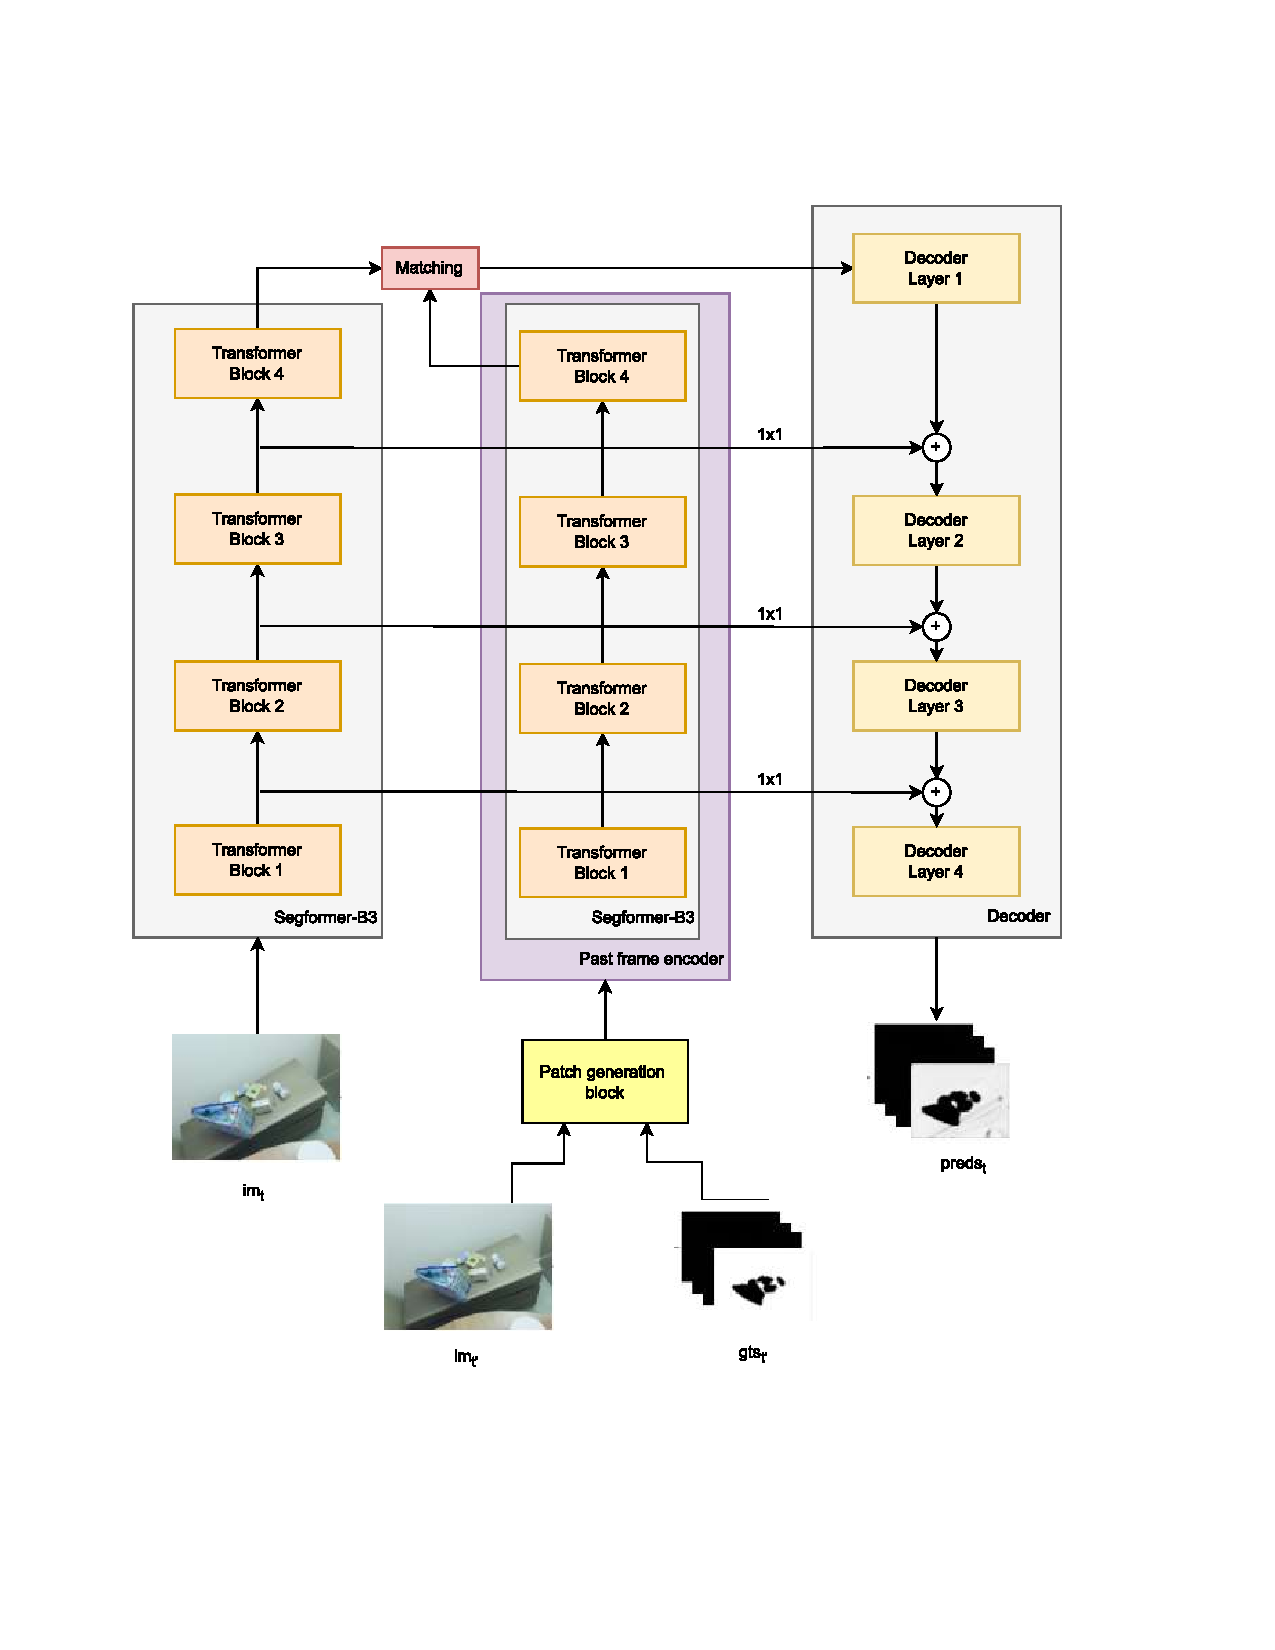
\includegraphics[width=1.\linewidth, trim={ 1cm 4cm 2.5cm 2cm}]{figures/03_method/model_detailed_backbone.pdf}
    \caption{Detailed model overview of the proposed backbone encoder 
    }
   
    \label{fig:detailed_model_backbone}
\end{figure}



\begin{figure}
    \centering
    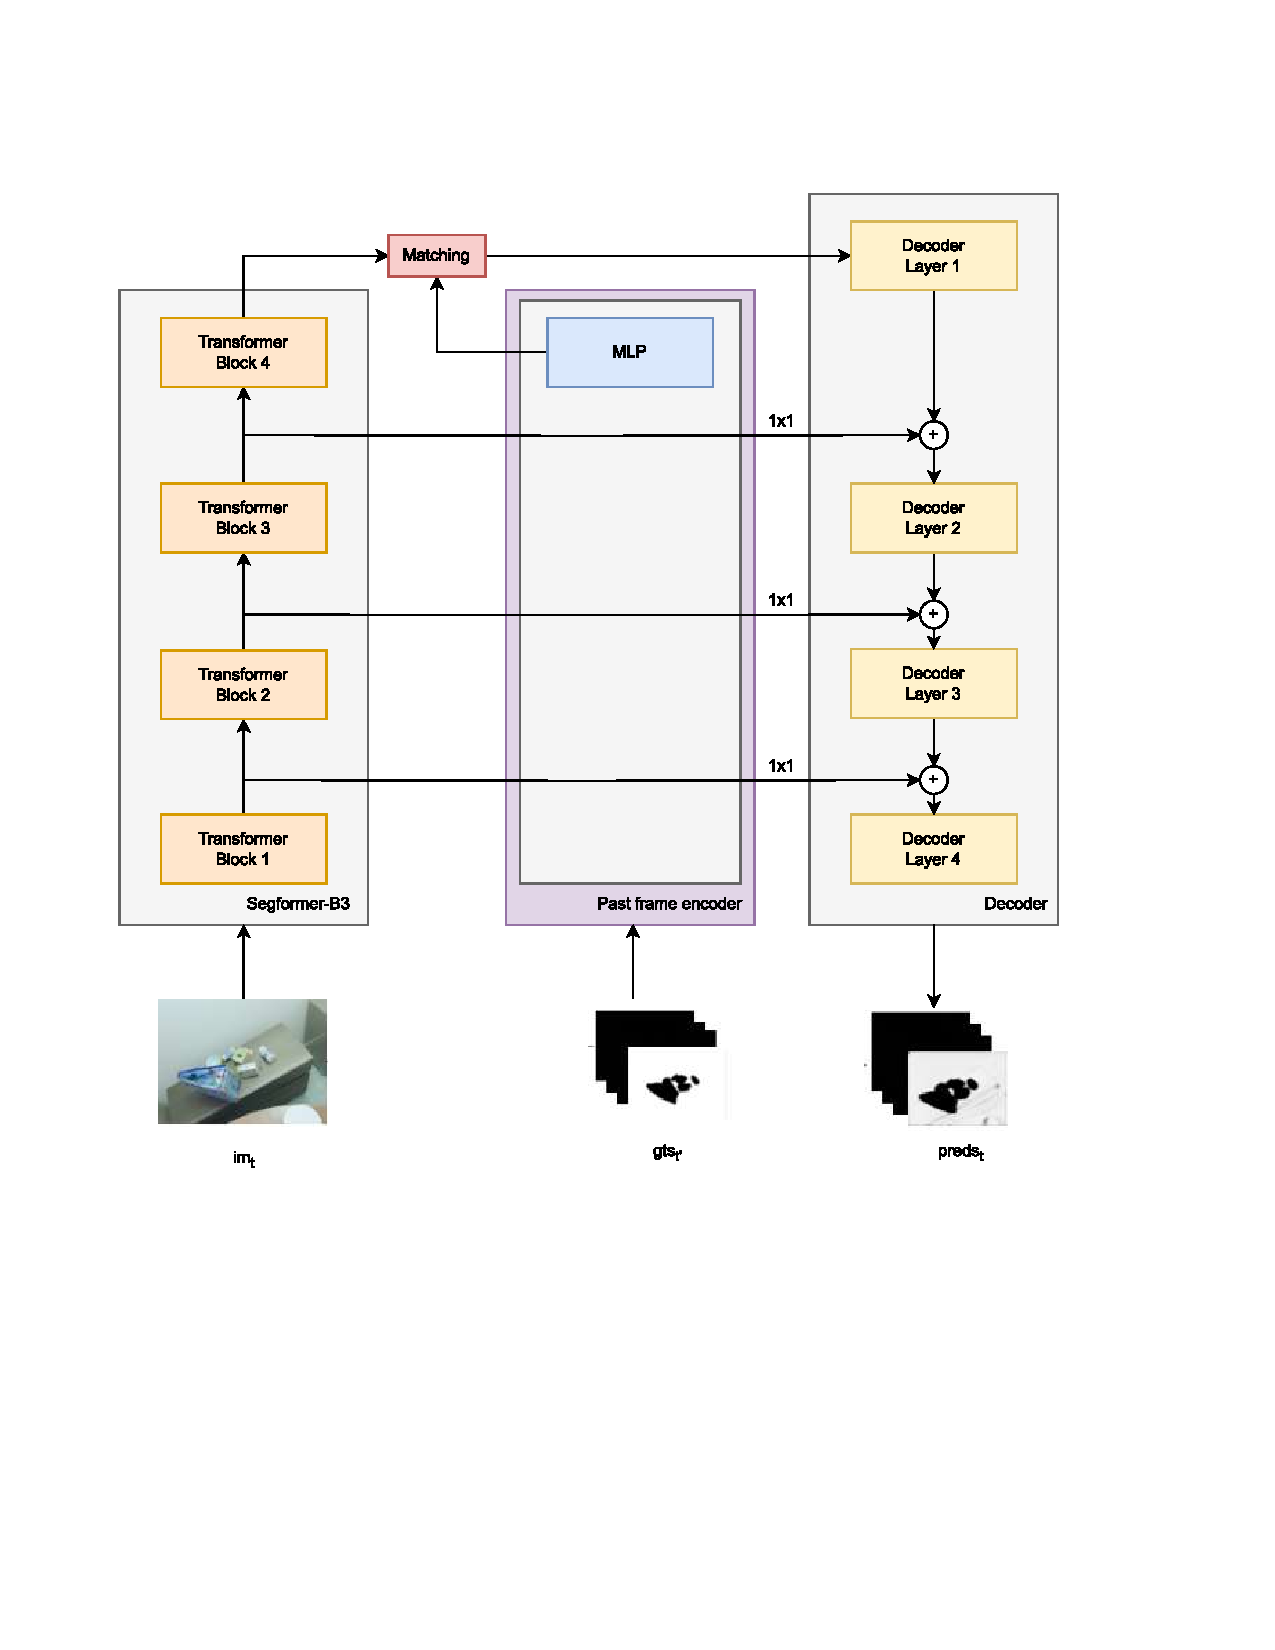
\includegraphics[width=1.\linewidth, trim={ 0.5cm 5cm 3cm 2cm}]{figures/03_method/model_detailed_bbox.pdf}
    \caption{Detailed model overview of the proposed bounding box encoder}
    \label{fig:detailed_model_bbox}
\end{figure}

\begin{figure}
    \centering
    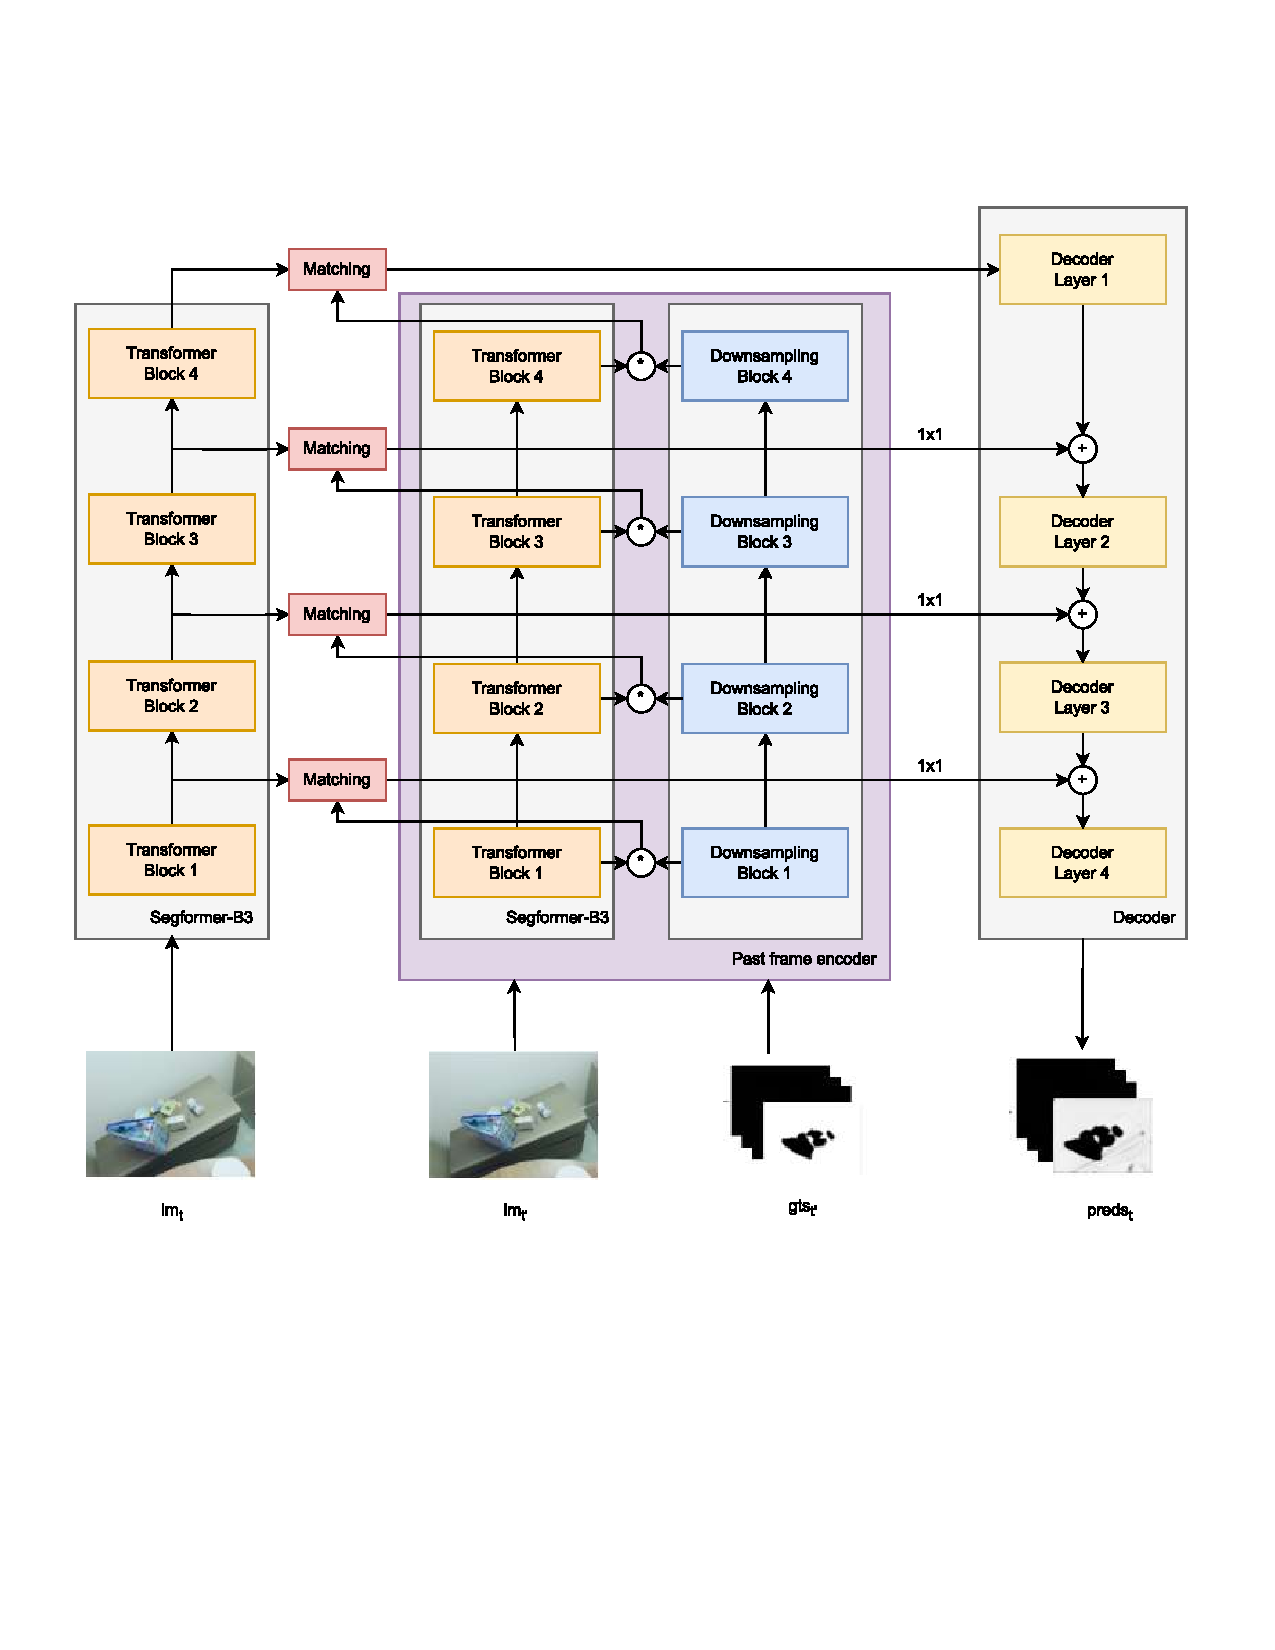
\includegraphics[width=1.\linewidth, trim={ 0.5cm 4cm 1cm 1.5cm}]{figures/03_method/model_detailed_overview.pdf}
    \caption{Detailed model overview of the proposed mask encoder
    % \comWB{its not entirely clear from the figure that only nonzero features are used during matching, how could we visualize this?}
    }
    \caption*{Note that the * operator is indicating a masking operation that results in feature cluster assignment}
    \label{fig:detailed_model}
\end{figure}

